\subsubsection{Opis przypadków użycia - klient}



Poniżej przedstawiono przypadki użycia związanie z procesowaniem i obsługą
danych klientów. We wszystkich (poza jednym) przypadkach aktorem jest sam
klient, jedynie wyrejestrowanie takiej osoby dokonywane jest przez uprawnionego
pracownika sklepu.



\begin{figure}[h!]
    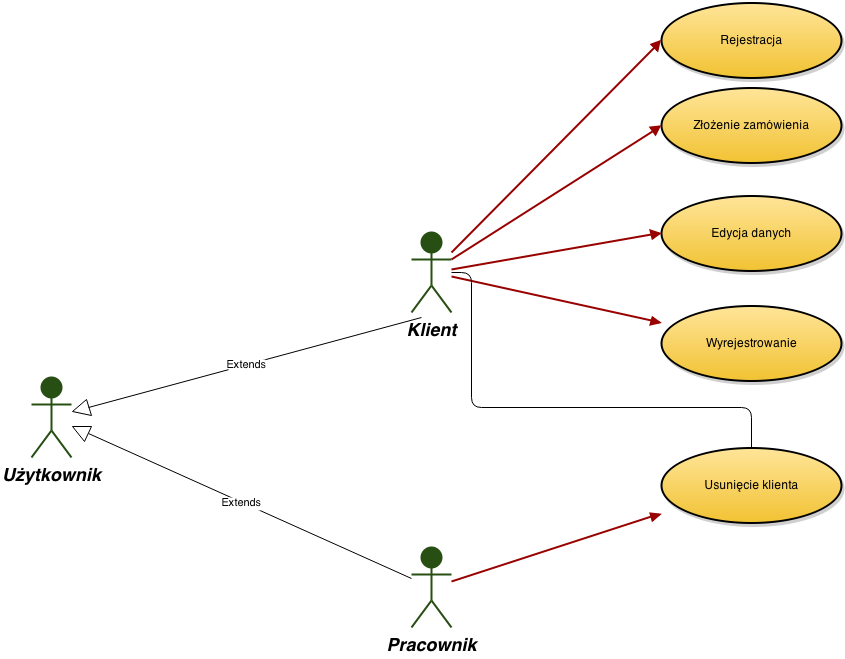
\includegraphics[width=\textwidth,
    height=0.5\textheight]{graphics/UseCase/Klient/UseCaseDiagram.png}
  \caption{Diagram przypadków użycia związanych z procesowaniem danych klienta}
\end{figure}





\newpage
\begin{enumerate}
   \item Rejestracja klienta - scenariusz główny \\
 
 Opis słowny - jest to pierwszy przypadek użycia dla klienta, bez którego
 pozostałe przypadki nie mają racji bytu. Akcje w nim opisane mają miejsce, gdy
 użytkownik pierwszy raz pojawia się na stronie i po przejrzeniu oferty sklepu
 (co dostępne jest także dla użytkowników niezalogowanych) decyduje się na
 stworzenie konta i ewentualne rozpoczęcie zakupów. Obsługa tego przypadku
 użycia wymaga poprawnego procesowania operacji rejestracji i jej potwierdzenia.
 
 \begin{longtable}{|p{5cm}|p{7cm}|}
 	\hline
	\textbf{Aktor} & Klient \\
	\hline
	\textbf{Warunki początkowe} & Klient niezalogowany, posiadający konto e-mail \\
	\hline
	\textbf{Opis przebiegu interakcji} & Wybór okna rejestracji, wypełnienie
	danych, potwierdzenia poprzez wiadomość e-mail \\
	\hline
	\textbf{Sytuacje wyjątkowe} & Klient już istniejący w bazie danych, brak konta
	e-mail \\
	\hline
	\textbf{Warunki końcowe} & Zarejestrowanie nowego klienta w systemie \\
	\hline
 \end{longtable}
 
  \item Rejestracja klienta - scenariusz główny \\
  \begin{tabularx}{\linewidth}{ c X}
  Aktor: & Klient \\
  \end{tabularx}
   \begin{enumerate}
    \item Klient uruchamia stronę internetową sklepu i wybiera opcję rejestracji
    \item Klient wstawia swoje dane osobowe i wybiera domyślny model płatności
    (kartą, za pobraniem itp.)
    \item System sprawdza wstawione dane (takie same hasła, czy istnieje już
    zarejestrowany w systemie użytkownik, czy istnieje podany adres e-mail itp.)
    \item System wysyła e-mail powitalny na adres podany przez klienta
    \item W ciągu określonego, zdefiniowanego czasu klient wybiera przesłany w
    e-mailu link, stając się pełnoprawnym użytkownikiem sklepu. Dane zapisywane
    są w bazie danych użytkowników a użytkownik może zalogować się  do systemu
  \end{enumerate}
  
  
  \item Rejestracja klienta - scenariusz alternatywny - klient już
  zarejestrowany w systemie \\
  \begin{tabularx}{\linewidth}{ c X}
  Aktor: & Klient \\
  \end{tabularx}
   \begin{enumerate}
     \item Kroki 1-2 scenariusza głównego
     \item System informuje użytkownika, że jest już zarejestrowany w systemie
     \item System przenosi użytkownika do ekranu logowania
   \end{enumerate} 
   
   \item Rejestracja klienta - scenariusz alternatywny - klient nie posiada
   adresu e-mail
   \begin{tabularx}{\linewidth}{ c X}
	Aktor: & Klient \\
  	\end{tabularx}   
  	\begin{enumerate}
  	  \item Kroki 1-4 scenariusza głównego
  	  \item System informuje użytkownika, że podany adres e-mail nie istnieje i
  	  przenosi użytkownika z powrotem do ekranu wypełniania danych wraz z
  	  adnotacją, by przed dalszą rejestracją założył konto e-mail.
  	\end{enumerate}
  	
  	
\item Rejestracja klienta - scenariusz alternatywny - klient nie klika w linka
aktywacyjny
   \begin{tabularx}{\linewidth}{ c X}
	Aktor: & Klient \\
  	\end{tabularx}   
  	\begin{enumerate}
  	  \item Kroki 1-5 scenariusza głównego
  	  \item System odrzuca prośbę użytkownika o rejestrację i nie umieszcza jego
  	  danych w bazie użytkowników. Przy następnym rozpoczęciu procesowania
  	  przypadku użycia Rejestracja Klienta klient musi od nowa wypełnić wszystkie
  	  dane. Do tego czasu nie może korzystać z opcji dostępnych tylko dla osób
  	  zalogowanych.
  	\end{enumerate}
  	
  	
  	
\begin{figure}[h!]
    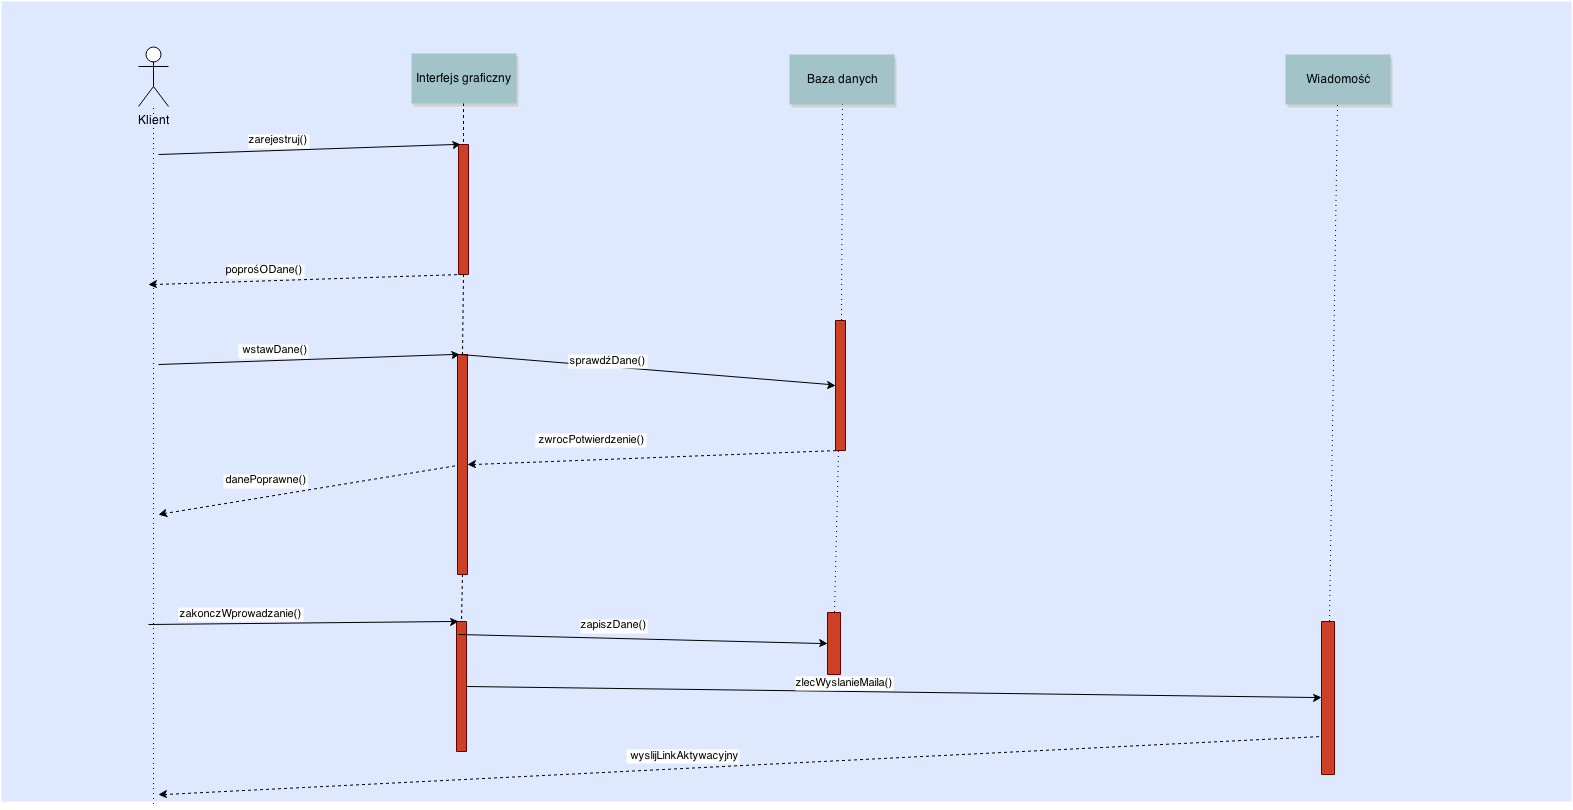
\includegraphics[width=\textwidth,
    height=0.5\textheight]{graphics/UseCase/Klient/RejestracjaKlientaSD.png}
  \caption{Diagram sekwencji dla przypadku użycia Rejestracja Klienta -
  scenariusz główny}
\end{figure}
  \item Złożenie zamówienia \\
 

 Opis słowny - jest to główny przypadek użycia, będący podstawową jednostką
 działania w niemal każdym sklepie internetowym. Złożenie zamówienia rozpoczyna
 się w momencie wyboru interesujących klienta towarów. Następnie zostaje on
 przekierowany do ekranu końcowego, gdzie wybiera sposób płatności i akceptuje
 zamówienie. Następnie zostaje do klienta wysłany e-mail potwierdzający
 
 \begin{longtable}{|p{5cm}|p{7cm}|}
 	\hline
	\textbf{Aktor} & Klient \\
	\hline
	\textbf{Warunki początkowe} & Klient zalogowany \\
	\hline
	\textbf{Opis przebiegu interakcji} & Wybór towarów, wybór sposobu płatności,
	akceptacja zamówienia \\
	\\
	\hline
	\textbf{Sytuacje wyjątkowe} & Użytkownik niezalogowany, użytkownik wycofuje się
	z  transakcji
	\\
	\hline
	\textbf{Warunki końcowe} & Nowe zamówienie w systemie \\
	\hline
 \end{longtable}


\item Złożenie zamówienia - scenariusz główny \\ 
  \begin{tabularx}{\linewidth}{ c X }
  Aktor: & Klient \\
  \end{tabularx}
  \begin{enumerate}
    \item Klient uruchamia stronę internetową sklepu i wyszukuje interesujące go
    produkty
    \item W momencie znalezienia pasującego produktu użytkownik wybiera opcję
    dodania do koszyka
    \item Po zakończeniu wyszukiwania użytkownik wybiera opcję przejścia do kasy
    \item System sprawdza, czy użytkownik jest zalogowany. 
    \item System sprawdza, czy użytkownik jest stałym klientem. Jeśli tak,
    dolicza rabat do ustalonej ceny (do sumy cen poszczególnych produktów)
    \item Użytkownik wybiera sposób płatności
    \item System dodaje do wcześniej ustalonej ceny koszty wynikające ze sposobu
    płatności
    \item Użytkownik wybiera sposób dostawy (poczta, kurier, odbiór osobisty
    itp.)
    \item System dodaje do ceny koszty wynikające ze sposobu dostawy
    \item Użytkownik, po sprawdzeniu wszystkich danych, decyduje się na złożenie
    zamówienia - po tym momencie nie może już ono być cofnięte
    \item System wysyła do użytkownika e-mail potwierdzający wraz z przewidywaną
    datą realizacji zamówienia
		
  \end{enumerate} 
  
  
  \item Złożenie zamówienia - scenariusz alternatywny - klient nie klika w linka
aktywacyjny
   \begin{tabularx}{\linewidth}{ c X}
	Aktor: & Klient \\
  	\end{tabularx}   
  	\begin{enumerate}
  	  \item Kroki 1-3 scenariusza głównego
  	  \item Jeśli użytkownik jest niezalogowany, system rozpoczyna procesowanie
  	  przypadku użycia Logowanie Do Systemu
  	  \item Po poprawnym zalogowaniu procesowanie przypadku użycia odbywa się jak
  	  w punktach 5-11
  	\end{enumerate}
  	
  	
  	\item Złożenie zamówienia - scenariusz alternatywny - klient rezygnuje z
  	zamówienia aktywacyjny
   \begin{tabularx}{\linewidth}{ c X}
	Aktor: & Klient \\
  	\end{tabularx}   
  	\begin{enumerate}
  	  \item Kroki 1-9 scenariusza głównego
  	  \item Użytkownik, po przeglądnięciu podsumowania całego zamówienia, nie
  	  decyduje się na złożenie zamówienia.
  	  \item System usuwa wszystkie dane tymczasowe z przeglądarki internetowej
  	  \item Pojawia się okno startowe sklepu internetowego
  	\end{enumerate}
  	
  	
   	
\begin{figure}[H]
    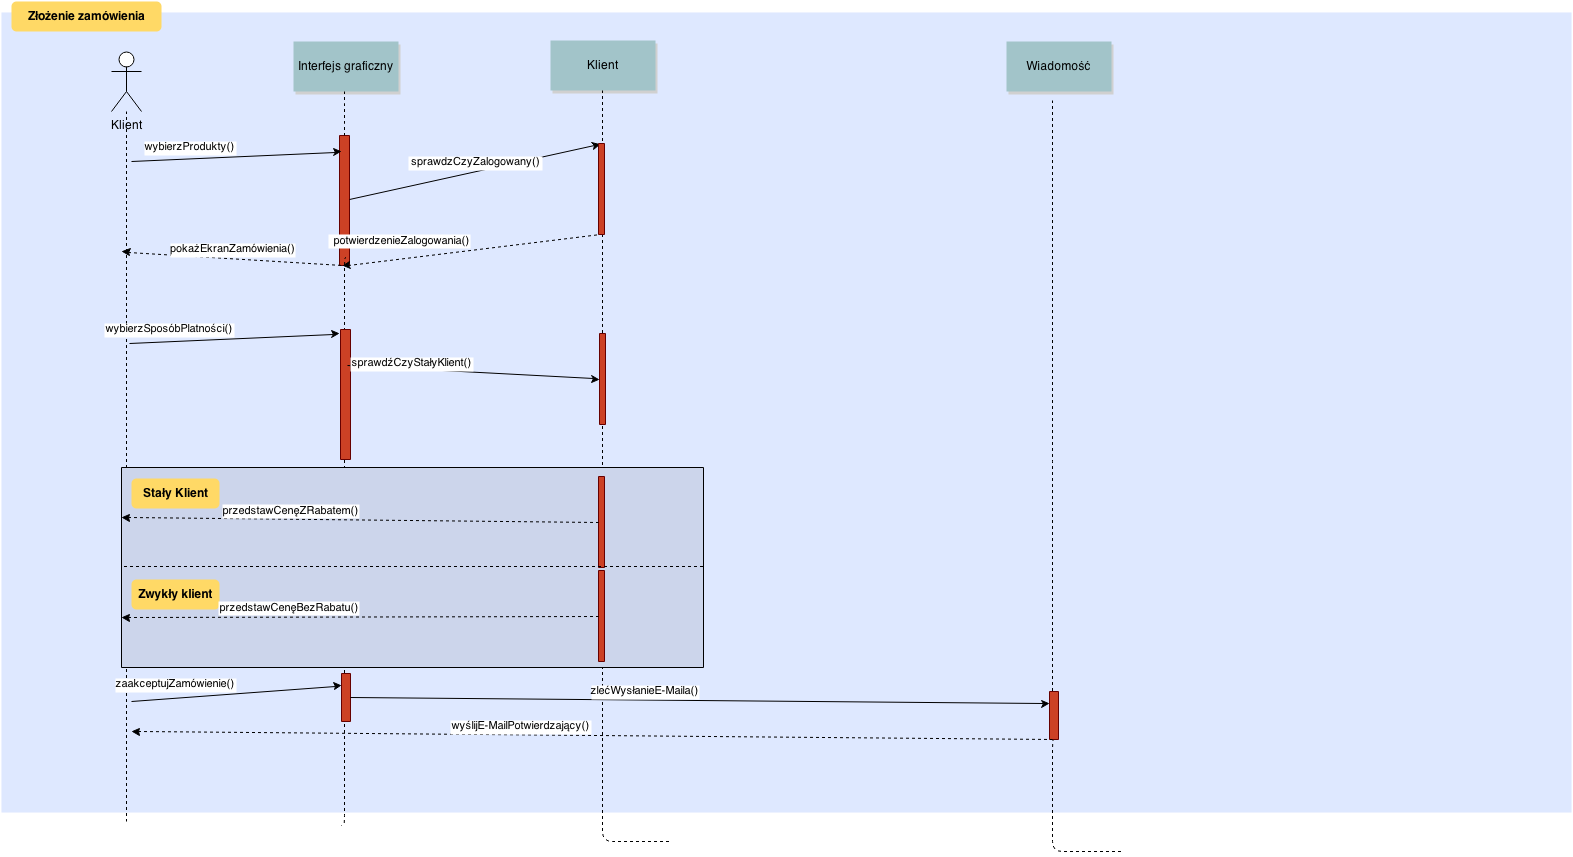
\includegraphics[width=\textwidth,
    height=0.5\textheight]{graphics/UseCase/Klient/ZlozenieZamowieniaSD.png}
  \caption{Diagram sekwencji dla przypadku użycia Złożenie Zamówienia -
  scenariusz główny}
\end{figure}
    \item Edycja danych klienta \\
 
 Opis słowny - przypadek użycia procesowany w momencie, gdy użytkownik (klient)
 zdecyduje się zmienić swoje dane, na przykład na skutek zmiany miejsca
 zamieszkania, adresu e-mail itp. Dane powinny być zapisane w bazie danych
 natychmiast po wprowadzeniu ich przez użytkownika i wszelkie zamówienia już
 realizowane a także te, które zostaną złożone w przyszłości
 
 \begin{longtable}{|p{5cm}|p{7cm}|}
 	\hline
	\textbf{Aktor} & Klient \\
	\hline
	\textbf{Warunki początkowe} & Klient zalogowany \\
	\hline
	\textbf{Opis przebiegu interakcji} & Zmiana danych w formularzu, zapis danych
	do bazy danych
	\\
	\hline
	\textbf{Sytuacje wyjątkowe} & Niepoprawne (nie takie same) wprowadzone hasła,
	zbyt krótkie hasło
	\\
	\hline
	\textbf{Warunki końcowe} & Poprawnie zmienione w bazie dane \\
	\hline
 \end{longtable}
 

 \item Edycja danych klienta - scenariusz główny \\
  \begin{tabularx}{\linewidth}{ c X }
  Aktor: & Klient \\
  \end{tabularx}
  \begin{enumerate}
    \item Klient uruchamia witrynę internetową sklepu
    \item Klient loguje się do systemu (tylko osoba zalogowana może zmieniać
    swoje dane)
    \item Klient edytuje wybrane pozycje ze swojego opisu (adres, numer
    telefonu itp.)
    \item W przypadku zmiany hasła klient proszony jest o podanie starego jak i
    nowego (dwukrotnie) hasła
    \item Klient zatwierdza wprowadzone zmiany
    \item System wysyła na podany przez użytkownika adres e-mail (nowy, jeśli
    to adres e-mail był jedną ze zmienianych wartości) informację o zmianie.
  \end{enumerate}
  
  
   \item Edycja danych klienta - scenariusz alternatywny - Niezgodne hasła\\
  \begin{tabularx}{\linewidth}{ c X }
  Aktor: & Klient \\
  \end{tabularx}
  \begin{enumerate}
    \item Kroki 1-4 jak w scenariuszu głównym
    \item W przypadku niezgodnych haseł system informuje użytkownika o błędzie
    wprowadzonych danych
    \item Jeśli niezgodność danych powtórzy się 3-krotnie, na e-mail użytkownika
    wysyłana jest informacja, że potencjalnie ktoś próbuje zmienić dane bez
    wiedzy upoważnionego użytkownika
  \end{enumerate}
  
  
  
  \begin{figure}[h!]
    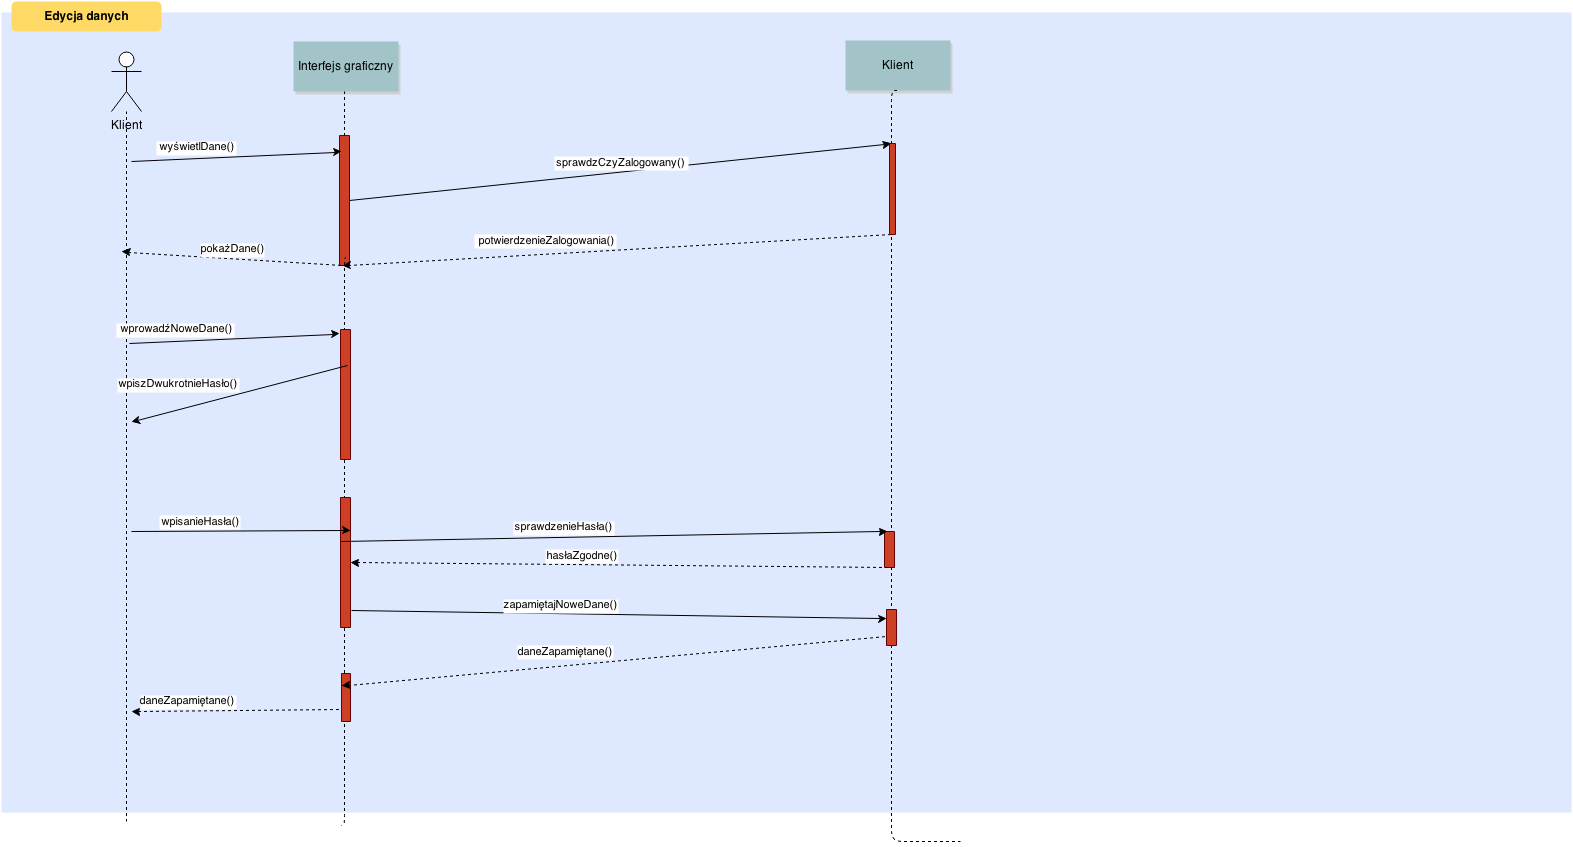
\includegraphics[width=\textwidth,
    height=0.5\textheight]{graphics/UseCase/Klient/EdycjaDanychKlientaSD.png}
  \caption{Diagram sekwencji dla przypadku użycia Edycja Danych Klienta -
  scenariusz główny}
\end{figure}
     \item Wyrejestrowanie się klienta \\
 
 Opis słowny - jest to pierwszy przypadek użycia dla klienta, bez którego
 pozostałe przypadki nie mają racji bytu. Akcje w nim opisane mają miejsce, gdy
 użytkownik pierwszy raz pojawia się na stronie i po przejrzeniu oferty sklepu
 (co dostępne jest także dla użytkowników niezalogowanych) decyduje się na
 stworzenie konta i ewentualne rozpoczęcie zakupów. Obsługa tego przypadku
 użycia wymaga poprawnego procesowania operacji rejestracji i jej potwierdzenia.
 
 \begin{longtable}{|p{5cm}|p{7cm}|}
 	\hline
	\textbf{Aktor} & Klient \\
	\hline
	\textbf{Warunki początkowe} & Klient zalogowany, posiadający konto w systemi \\
	\hline
	\textbf{Opis przebiegu interakcji} & Podjęcie decyzji o wyrejestrowaniu,
	obsługa aktywnych zamówień
	\\
	\hline
	\textbf{Sytuacje wyjątkowe} & Brak\\
	\hline
	\textbf{Warunki końcowe} & Usunięcie klienta z systemu\\
	\hline
 \end{longtable}
 
  
  
  \item Wyrejestrowanie się klienta - scenariusz główny\\
  \begin{tabularx}{\linewidth}{ c X }
  Aktor: & Klient \\
  \end{tabularx}
  \begin{enumerate}
    \item Klient uruchamia witrynę internetową i loguje się na swoje konto
    (przypadek użycia Logowanie Do Systemu)
    \item Klient wybiera opcję usunięcia danych
    \item System sprawdza, czy istnieją niezrealizowane (oczekujące) zamówienia.
    Jeśli tak, wyświetla się alert z informacją, czy dane zamówienie zostało już
    wcześniej opłacone
    \item Jeśli istniały już zamówienia, które zostały opłacone a nie zostały
    jeszcze zrealizowane, system zleca odesłanie określonej kwoty pieniężnej z
    powrotem na konto użytkownika (z pominięciem kosztów obsługi)
    \item Klient zostaje poproszony o podanie przyczyn swojej decyzji -
    wypełnianie jest nieobowiązkowe
    \item Dane przechowywane są przez Okres Przechowywania Danych (wymaganie
    prawne - patrz Wymagania niefunkcjonalne punkt \ref{itm:OPD}). W tym
    czasie klient może ponownie zarejestrować się w systemie bez utraty poprzednich danych
    \item W przypadku braku ponownej rejestracji dane zostają na stałe usunięte
    z firmowej bazy danych
  \end{enumerate}
  
  
  
  \begin{figure}[H]
    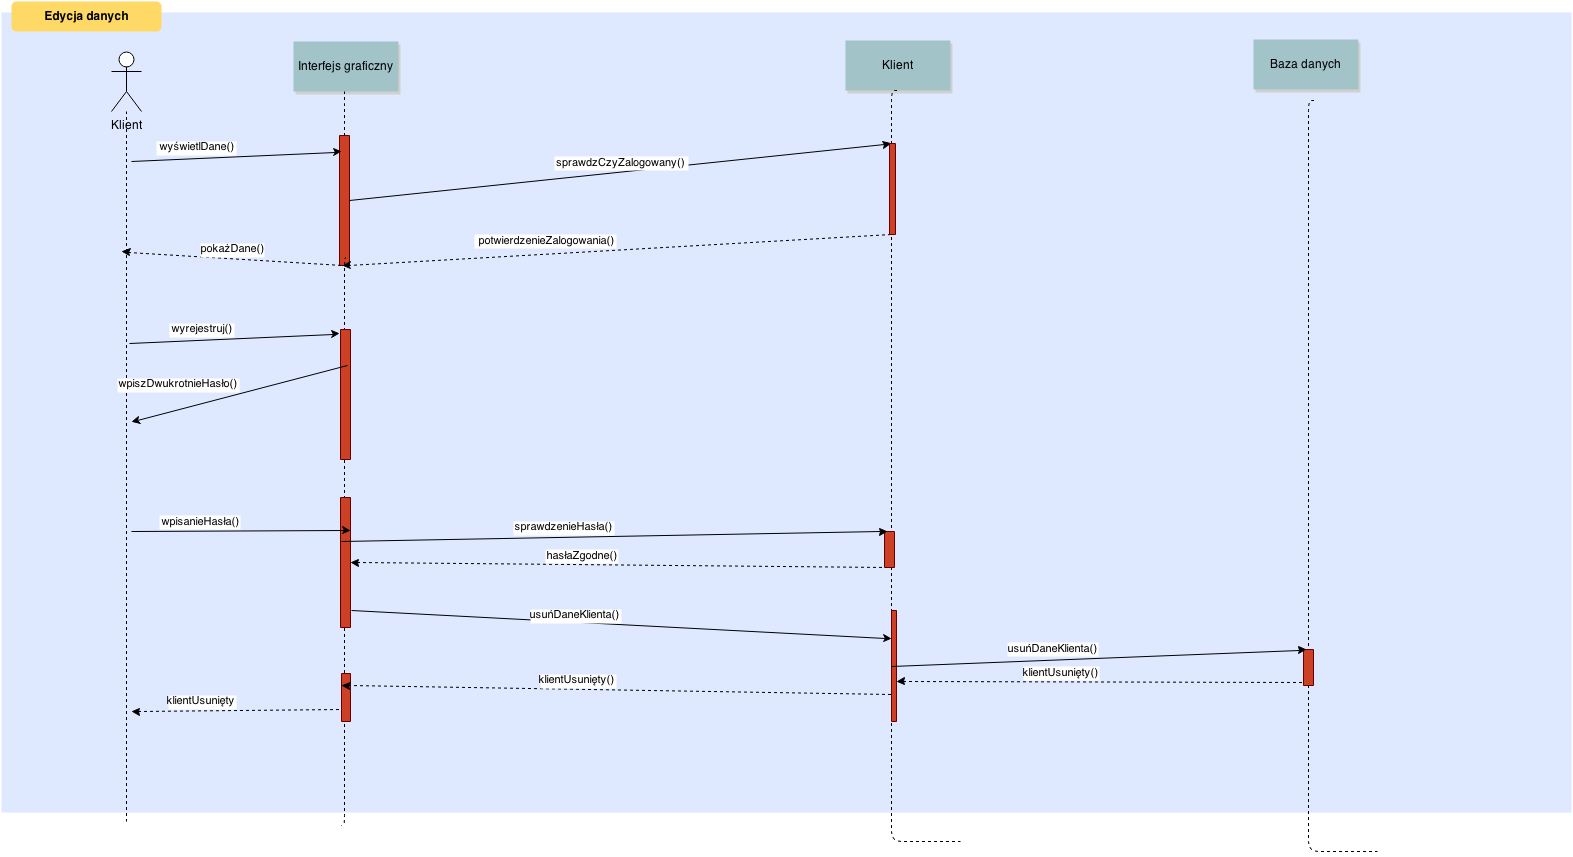
\includegraphics[width=\textwidth,
    height=0.5\textheight]{graphics/UseCase/Klient/WyrejestrowanieSieKlientaSD.png}
    \caption{Diagram sekwencji dla przypadku użycia Wyrejestrowanie Się Klienta
    - scenariusz główny}
\end{figure}
  
  
 
  \item Usunięcie klienta \\
  \begin{tabularx}{\linewidth}{ c X }
  Aktor: & Pracownik \\
  Opis: & Klienta można usunąć administracyjnie na przykład z powodów
  naruszenia regulaminu.\\
  \end{tabularx}
  \begin{enumerate}
    \item Pracownik sklepu wyszukuje klienta o konkretnym imieniu i nazwisku
    (lub według innych kryteriów)
    \item Pracownik wybiera opcję usunięcia klienta. 
    \item Pracownik wpisuje powód, dla którego usuwa użytkownika (informacja ta
    będzie przesłana do klienta w wiadomości e-mail)
    \item Pracownik wypełnia dane dotyczące kwestii niezrealizowanych zamówień i
    nieotrzymanych płatności
    \item Obie informacji (z poprzednich 2 kroków) są przekazywane na podany
    przez użytkownika adres e-mail
    \item Dane są przechowywane przez Okres Magazynowania Danych (patrz
    Wymagania Niefunkcjonalne punkt \ref{itm:OMD}) - w tym czasie użytkownik
    może złożyć reklamację i ewentualnie odzyskać dostęp do konta
    \item Po tym czasie, jeśli prośba o przywrócenie konta nie zostanie
    pozytywnie rozpatrzona, dane są na stałe usuwane z systemu
  \end{enumerate}
\end{enumerate} 
 
\newpage
\begin{figure}[H]
    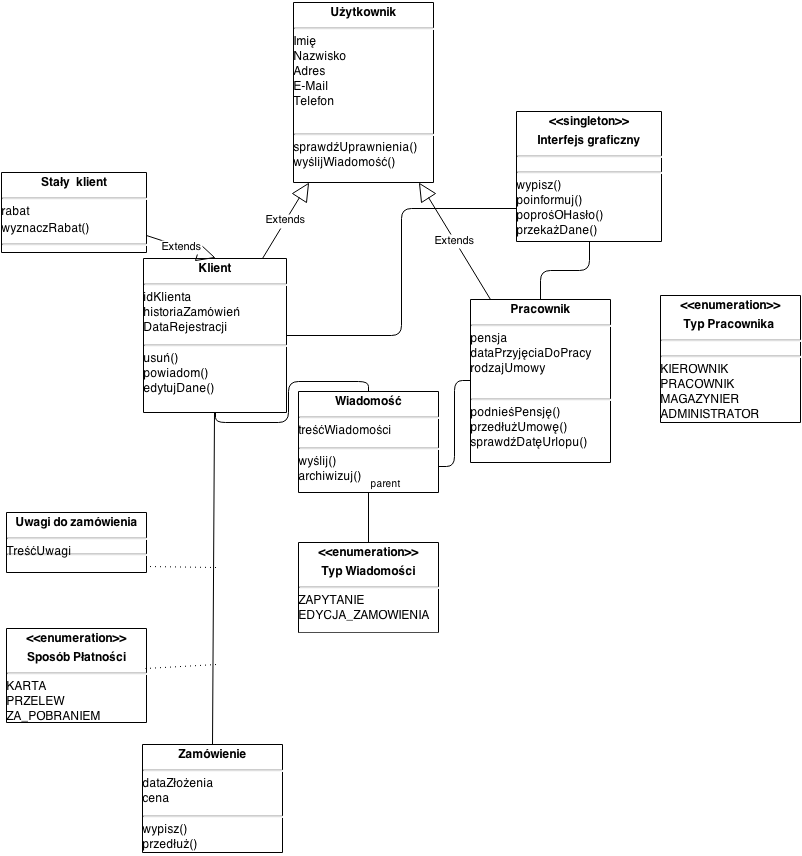
\includegraphics[width=\textwidth,
    height=\textheight]{graphics/UseCase/Klient/KlientClassDiagram.png}
  \caption{Diagram klas wykorzystywanych przy procesowaniu przypadków użycia
  związanych z klientem}
\end{figure} 


